\item \textbf{Now, explore whether you can leverage additional information in the file as exogenous variables. Use appropriate tools to evaluate the suitability of using these variables and summarize your results. There is no fixed number of variables assigned – use your judgement and justify your decisions.  Using an ARIMAX framework, show the impact of including additional variables as part of your prediction. Repeat the analysis in 2 (a) and (b) using the updated models.} 


\textit{First, we visualized the raw signals.} 

\begin{figure}[H]
    \centering
    \begin{minipage}[b]{1\textwidth}
        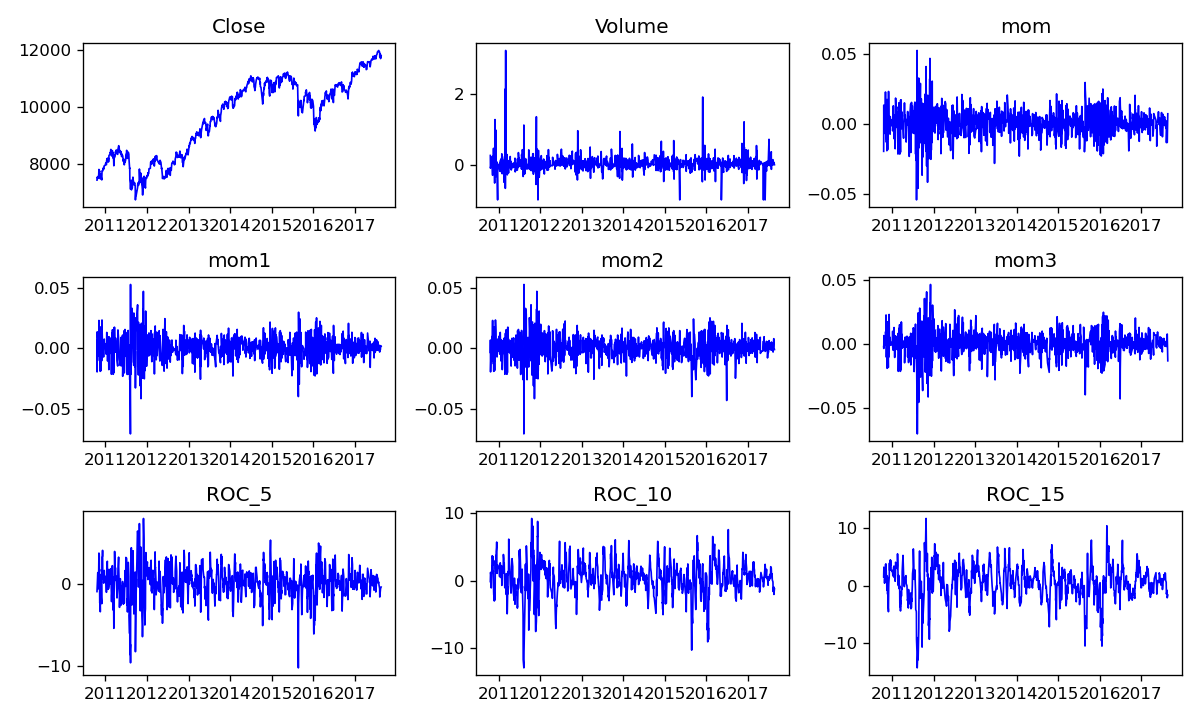
\includegraphics[width=\textwidth]{figures/Ass2/Ass2_Q3_raw_signal.png}
    \end{minipage}
    \caption{The visualization of the first nine columns.}
    \label{fig:Ass2_Q3_raw_signal}
\end{figure}




\textit{As these signals had the different range, we used standardization to transform all data to range -1 and 1. Figure \ref{fig:Ass2_Q3_standard_data} indicates the standardized signals. Also, we applied \gls{ADF} on these signals to find out that these signals were stationary or non-stationary. Table \ref{tab:Ass2_Q3_ADF_results} shows the result of this test on the dataset.}

\begin{figure}[H]
    \centering
    \begin{minipage}[b]{1\textwidth}
        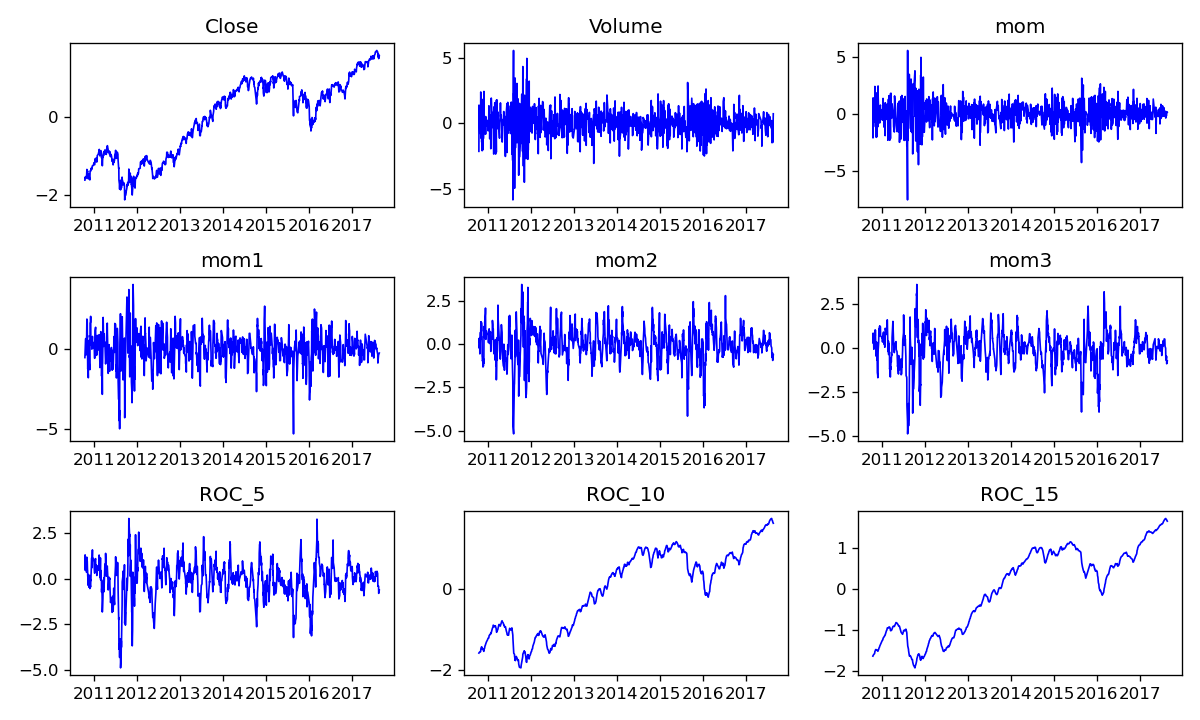
\includegraphics[width=\textwidth]{figures/Ass2/Ass2_Q3_standard_data.png}
    \end{minipage}
    \caption{A plot of \gls{ACF} and \gls{PACF} of the dataset.}
    \label{fig:Ass2_Q3_standard_data}
\end{figure}


\begin{table}[H]
\centering
\caption{The result of the \gls{ADF} on the dataset.}
\label{tab:Ass2_Q3_ADF_results}
{\scriptsize
\begin{tabular}{lrrrrrrrrr}
\toprule
{} &        Close &        Volume &           mom &         mom1 &          mom2 &         mom3 &         ROC\_5 &        ROC\_10 &        ROC\_15 \\
\midrule
ADF Statistic               &    -1.08 & -14.88 & -12.13 &   -38.46 & -8.14 &   -20.97 & -10.61 & -9.75 & -6.99 \\
p-value                     &     0.720 &  1.5e-27 &  1.7e-22 &     0.00 &  9.8e-13 &     0.00 &  5.5e-19 &  7.9e-17 &  7.5e-10 \\
\#Lags Used                  &     2 &  4 &  11 &     0 &  20 &     2 &  9 &  6 &  16 \\
Number of Obs Used &  1111 &  1109 &  1102 &  1113 &  1093 &  1111 &  1104 &  1107 &  1097 \\
Critical Value (1\%)         &    -3.436 & -3.436 & -3.436 &    -3.436 & -3.436 &    -3.436 & -3.436 & -3.436 & -3.436 \\
Critical Value (5\%)         &    -2.864 & -2.864 & -2.864 &    -2.864 & -2.864 &    -2.864 & -2.864 & -2.864 & -2.864 \\
Critical Value (10\%)        &    -2.568 & -2.568 & -2.568 &    -2.568 & -2.568 &    -2.568 & -2.568 & -2.568 & -2.568 \\
\bottomrule
\end{tabular}
}
\end{table}

\textit{According to table \ref{tab:Ass2_Q3_ADF_results} all columns were stationary except the "Close price".  
We used a first-order differencing to turn this time series to a stationary data. Figures \ref{fig:Ass2_Q3_1diff_Close_signal} and \ref{fig:Ass2_Q3_PACF_ACF_1diff} indicate this $1^{st}$ order differencing signal along with its \gls{ACF} and \gls{PACF} plots. These two plots also show that the data got stationary.}

\begin{figure}[H]
    \centering
    \begin{minipage}[b]{1\textwidth}
        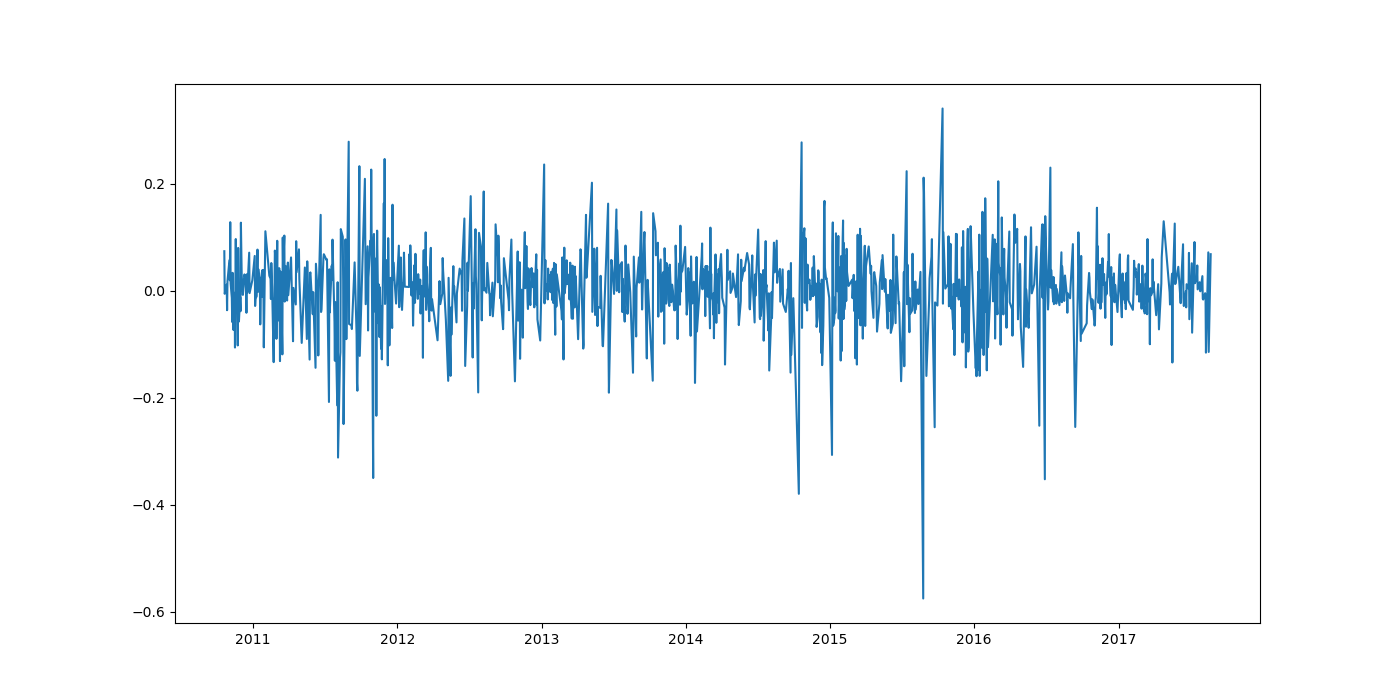
\includegraphics[width=\textwidth]{figures/Ass2/Ass2_Q3_1diff_Close_signal.png}
    \end{minipage}
    \caption{The $1^{st}$ order differencing of "Close price" data.}
    \label{fig:Ass2_Q3_1diff_Close_signal}
\end{figure}

\begin{figure}[H]
    \centering
    \begin{minipage}[b]{1\textwidth}
        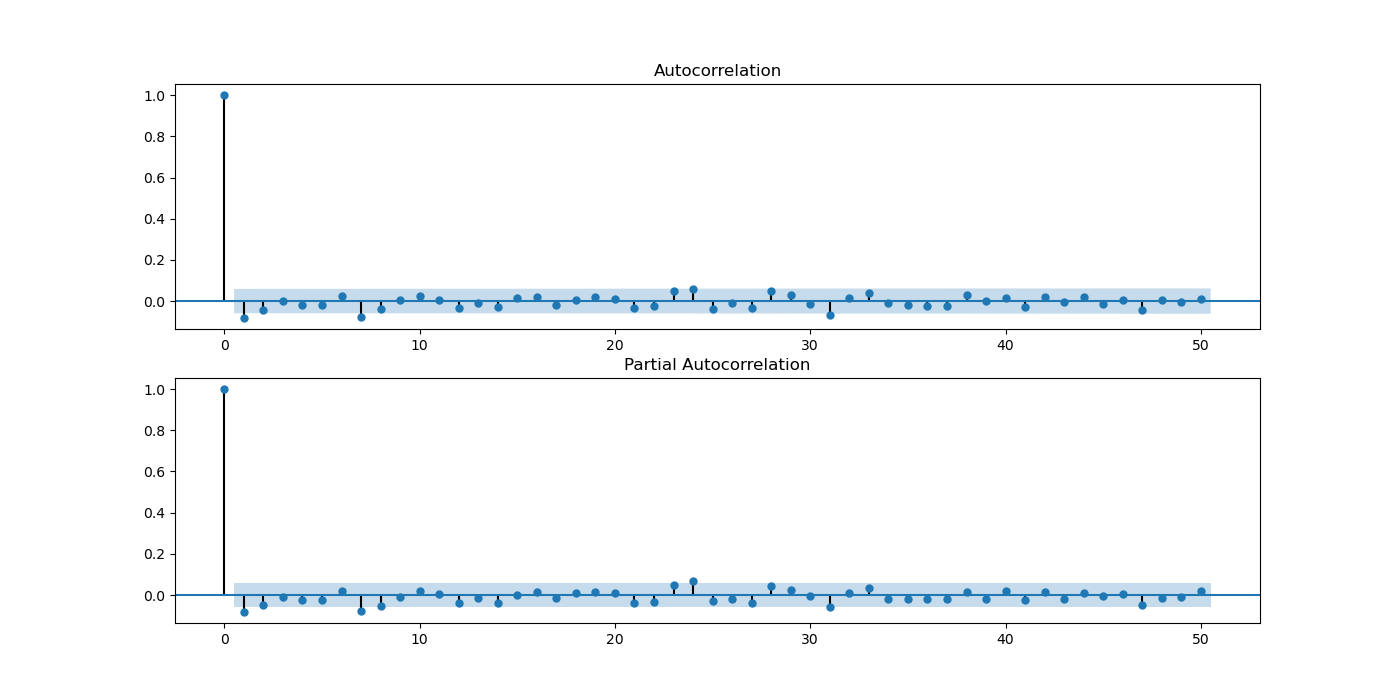
\includegraphics[width=\textwidth]{figures/Ass2/Ass2_Q3_PACF_ACF_1diff.png}
    \end{minipage}
    \caption{A plot of \gls{ACF} and \gls{PACF} on the $1^{st}$ order differencing in "Close price".}
    \label{fig:Ass2_Q3_PACF_ACF_1diff}
\end{figure}

\textit{After transforming and making stationary, we applied 
Granger causality test on data. The null hypothesis (H0) of this test says that two variables does not Granger causes, and its alternate hypothesis (H1) indicates the second signal have a significant effect on the first signal. So where ever P-value is less than 0.05, we can consider Grange causality. Table \ref{tab:Ass2_Q3_Granger_results} indicates the result of this test on the first nine columns. For this test, the maximum lag set 30.\\
Based on this test, signals mom, mom1, mom2, and ROC\_X were Granger causality of the "Close price". Then these signals shifted as much as the corresponding lag, and were stored to feed to our model.}




\begin{table}[H]
\centering
\caption{The result of the \gls{ADF} on the dataset.}
\label{tab:Ass2_Q3_Granger_results}
{\footnotesize
\begin{tabular}{lrrrrrrrrr}
\toprule
{} &  Close &   Volume &      mom &     mom1 &     mom2 &    mom3 &   ROC\_5 &   ROC\_10 &   ROC\_15 \\
\midrule
min p\_value &    1.0 &   0.1634 &   0.0001 &   0.0033 &   0.0013 &  0.0919 &  0.0485 &   0.0068 &   0.0172 \\
lag         &    1.0 &  22 &  28 &  30 &  30 &  1 &  1 &  19 &  22 \\
Causality   &    0.0 &   0 &   1 &   1 &   1 &  0 &  1 &   1 &   1 \\
\bottomrule
\end{tabular}
}
\end{table}

\textit{The order of the model for this question was similar to the last question. Figure \ref{fig:Ass2_Q3_residual_plot} indicates the residual of fitted model. As this plot illustrates, the residual signal of model had a Gaussian distribution with zero mean. In addition, the \gls{ACF} plot shows that this signal is a stationary signal.}



\begin{figure}[H]
    \centering
    \begin{minipage}[b]{1\textwidth}
        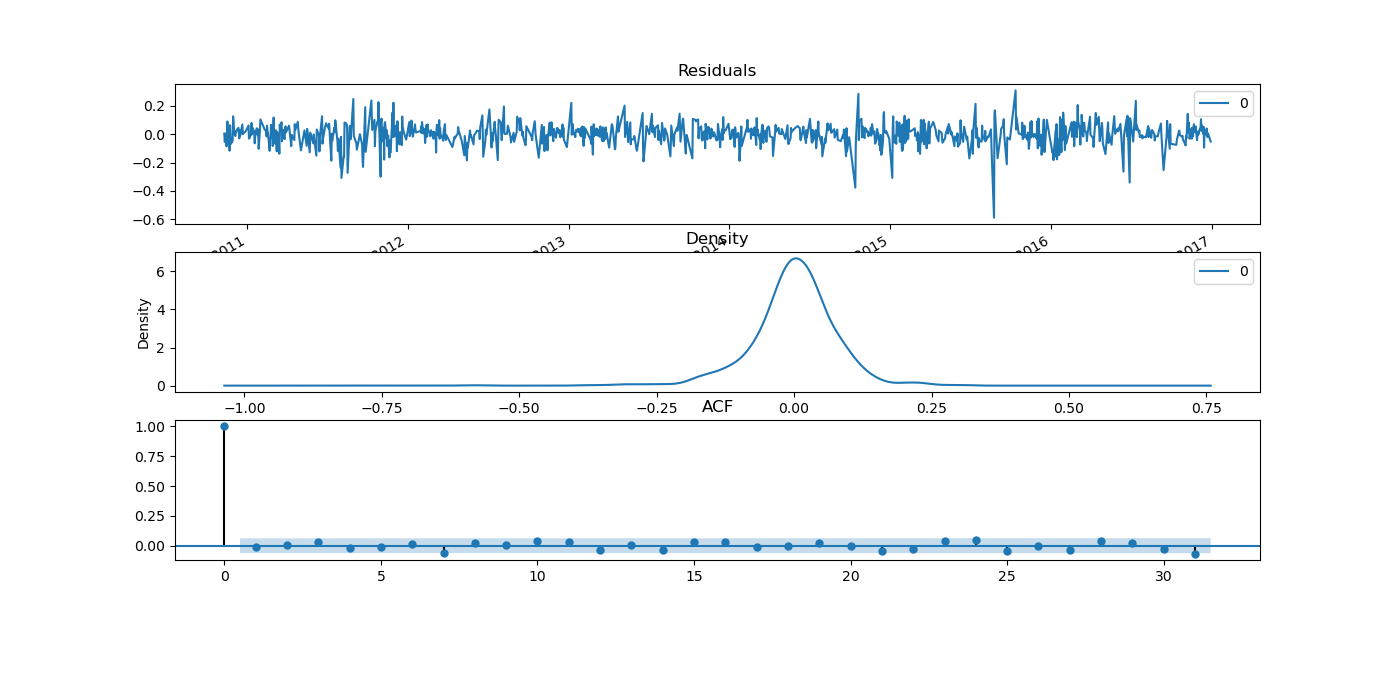
\includegraphics[width=\textwidth]{manuscript/src/figures/Ass2/Ass2_Q3_residual_plot.png}
    \end{minipage}
    \caption{The residual of the fitted model (\gls{arima}X(1, 0, 1)).}
    \label{fig:Ass2_Q3_residual_plot}
\end{figure}

\textit{To forecast, we split data into test and train set like the part 2. After prediction, we needed to reverse all transforms to get the real forecast. Figure \ref{fig:Ass2_Q3_Forecast_vs_Actuals} demonstrates the output of the fitted model. As can be seen, the model could predict like the \gls{arima} (question 2a), and because of using the exogenous variables, the prediction had some ripples that followed the the actual data. These ripples decreased the RMS error to 271.592.} 

\begin{figure}[H]
    \centering
    \begin{minipage}[b]{1\textwidth}
        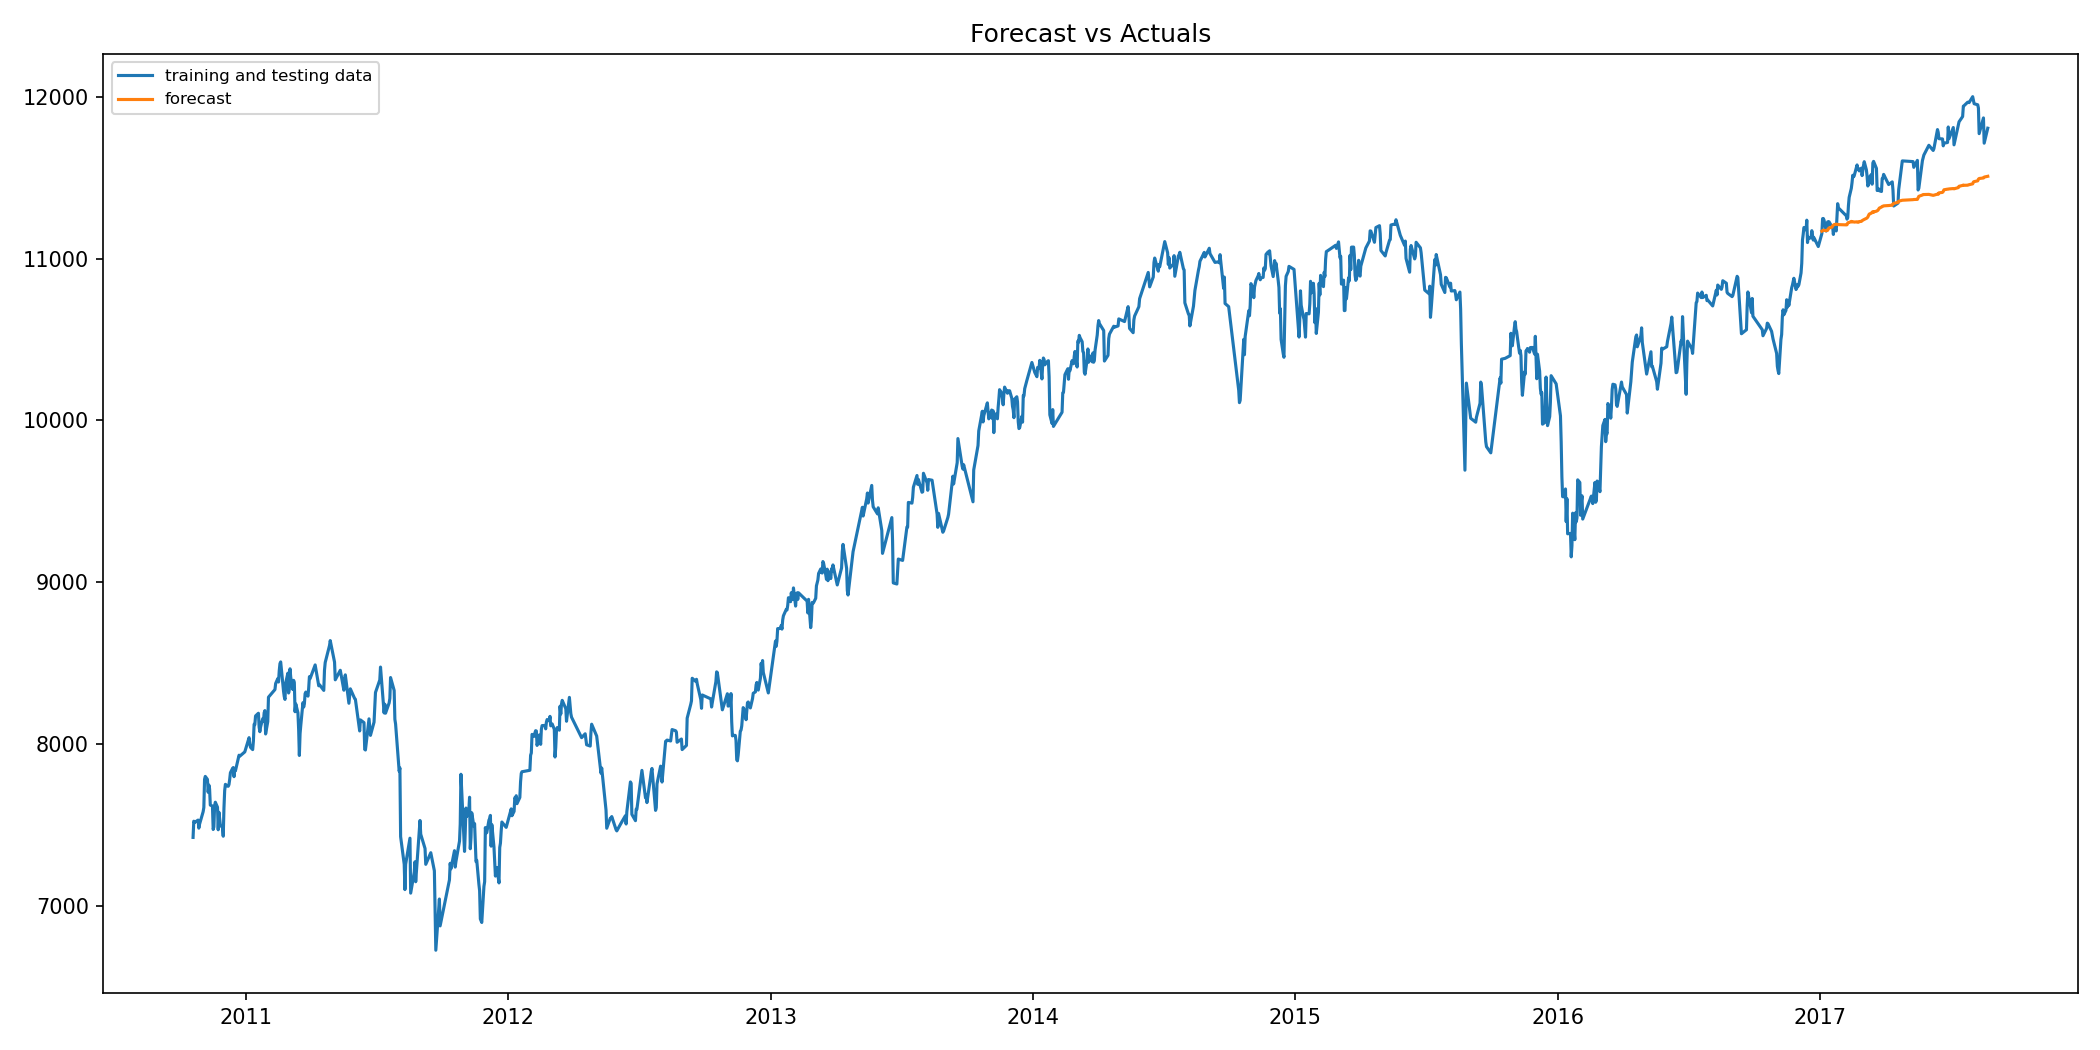
\includegraphics[width=\textwidth]{manuscript/src/figures/Ass2/Ass2_Q3_Forecast_vs_Actuals.png}
    \end{minipage}
    \caption{The prediction and actual data of \gls{arima}X(1, 0, 1) model.}
    \label{fig:Ass2_Q3_Forecast_vs_Actuals}
\end{figure}





\textit{For the rolling window approach, we used the same procedure in question 2. Figure \ref{fig:Ass2_Q3_Rolling_Forecast_vs_Actuals} demonstrates the output of the rolling window model for \gls{arima}X. As can be seen, the model could follow the the test set better than previous models. The RMS error decreased to 261.581. Since we used additional information of exogenous variables, the prediction had some ripples.}

\begin{figure}[H]
    \centering
    \begin{minipage}[b]{1\textwidth}
        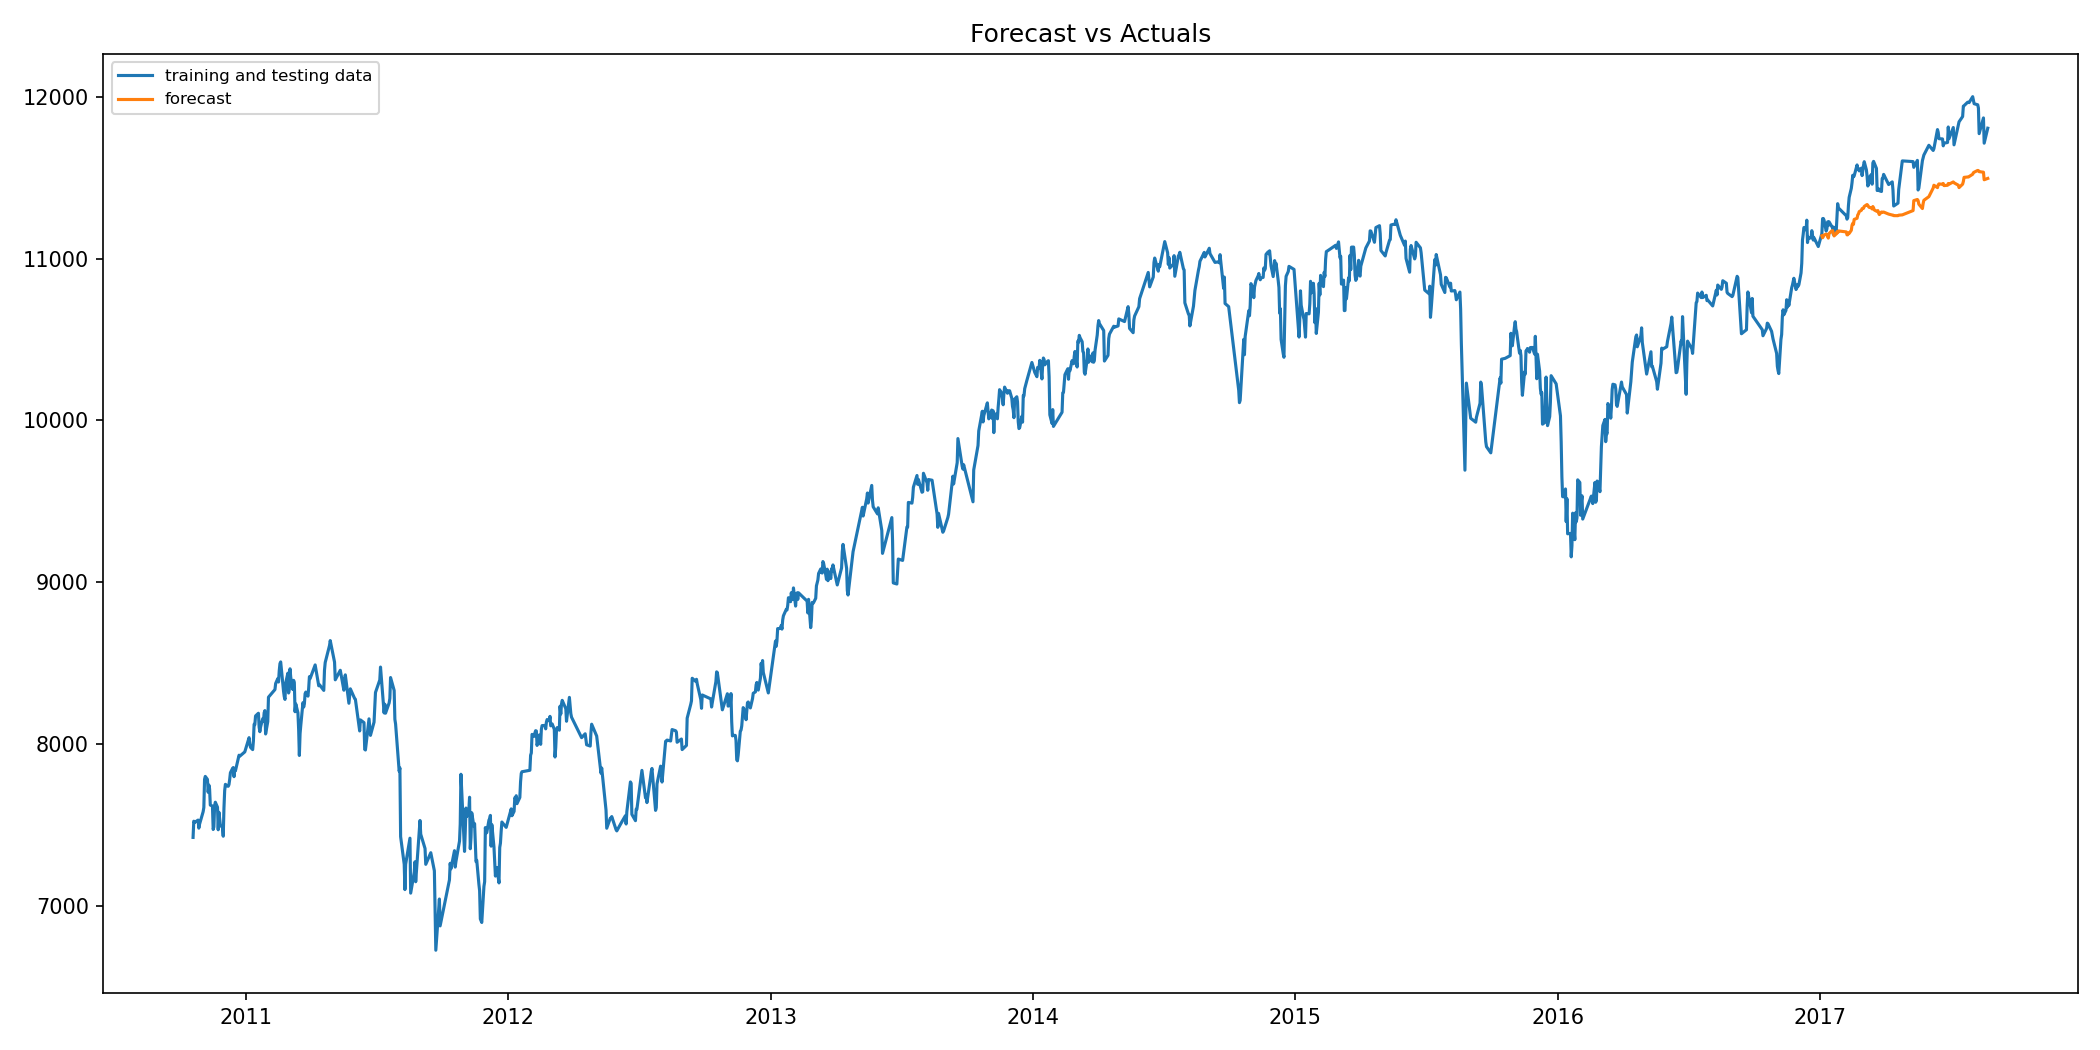
\includegraphics[width=\textwidth]{manuscript/src/figures/Ass2/Ass2_Q3_Rolling_Forecast_vs_Actuals.png}
    \end{minipage}
    \caption{The prediction and actual data of \gls{arima}X(1, 0, 1) model in rolling windows approach.}
    \label{fig:Ass2_Q3_Rolling_Forecast_vs_Actuals}
\end{figure}








